
\section{Сведение кратного интеграла к повторному}
\subsection{Двойные интегралы}
\setcounter{theorem}{0}
$\mathbb{E}^2, Oxy, \Pi=\{(x,y): a<x<b, c<y<d \} $
\begin{theorem}
	Пусть функция $\omega=f(x,y) $ определена на $\overline{\Pi}$ и интегрируема на $\Pi$ и выполнено:  $\forall x\in [a,b] \; \exists \; \mathbb{J}(x)=\int_c^d F(x,y) dy $ тогда функция $\mathbb{J}(x)$ интегрируема на $[a,b]$ и существует повторный интеграл: \\
	$$ \int_a^b \mathbb{J}(x)dx = \int_{a}^{b} dx \int_c^d f(x,y) dy \text{ и } \int_a^b dx \int_c^d f(x,y) dy = \iint_\Pi d(x,y) dxdy $$ 
\end{theorem}
\begin{proof}
	$a=x_0<x_1<\dots <x_k=b, \; c=y_0<y_1<\dots < y_n=d$\\
	$\Pi_{ij}=(x_{i-1}, x_{i})\times(y_{j-1}, y_j), i=\overline{1,k}, j=\overline{1,n} $\\
	$\{\Pi_{ij} \} $ - разбиение $\Pi; \; \Delta_x^i=x_i-x_{i-1}, i=\overline{1,k}; \Delta_y^j=y_j-y_{j-1}, j=\overline{1,n}$\\
	$\xi_i\in [x_{i-1}, x_i]  $ в $\overline{\Pi}_{ij}$ выполнено $(inf)\; m_{ij} \leq f(\xi_i, y) \leq M_{ij} \;(sup) $\\
	$\sum_{j=1}^n m_{ij} \Delta^j_y \leq \mathbb{J}(\xi_i)\leq  \sum_{j=1}^n M_{ij} \Delta^j_y  \Rightarrow \\
	\sum_{i=1}^k\sum_{j=1}^n m_{ij} \Delta_y^j \Delta_x^i \leq \sum_{i=1}^k\mathbb{J}(\xi_i) \Delta_x^i\leq \sum_{i=1}^k\sum_{j=1}^n M_{ij} \Delta_y^j \Delta_x^i; \;
	\Delta_T \rightarrow 0
	$
\end{proof}


\begin{determenition}
	Область $\Omega\subset \mathbb{E}^2$ называется \textbf{элементарной относительно Oy}, если ее граница состоит из графиков двух функций: $y=\phi(x);\; y=\psi(x) $ и, быть может, отрезков прямых  $x=a; \; x=b, $ при этом $\forall x\in [a,b] \rightarrow  \psi(x) \leq \phi(x).$
\end{determenition}

\begin{theorem}
	Пусть $\omega=f(x,y)$ непрерывна на $\overline{\Omega} $ и область $\Omega$ элементарна относительно оси $Oy$, ее граница состоит из двух графиков непрерывных функций $y=\phi(x);\; y=\psi(x) $ и, быть может, отрезков прямых $x=a; \; x=b $, причем $\forall x\in [a,b] \rightarrow  \psi(x) \leq \phi(x).$ Тогда существует повторный интеграл $\int_a^b dx \int_{\psi(x)}^{\phi(x)} f(x,y) dy = \iint_{\Omega} f(x,y) dxdy $
\end{theorem}
\begin{proof}
	\textbf{Замечание:} из условия теоремы следует, что: 
	\begin{enumerate}
		\item $\Omega $ - измеримая область
		\item $f$ - интегрируема на $\Omega$
		\item При фикс $x$  функция $ f$ неперерывна по переменной $y$. И $f$ интегрируема на $[\phi(x), \psi(x)] $
	\end{enumerate}
	
	Пусть $\Pi$ такой прямоугольник, что $\overline{\Omega}\subseteq \overline{\Pi} $
	Тогда: $f(x,y)=\begin{cases}
		f(x,y)&, (x,y) \in \overline{\Omega}\\
		0&, (x,y) \in  \overline{\Pi}\backslash \overline{\Omega}
	\end{cases}$
	
\end{proof}

	\begin{figure}[H]
	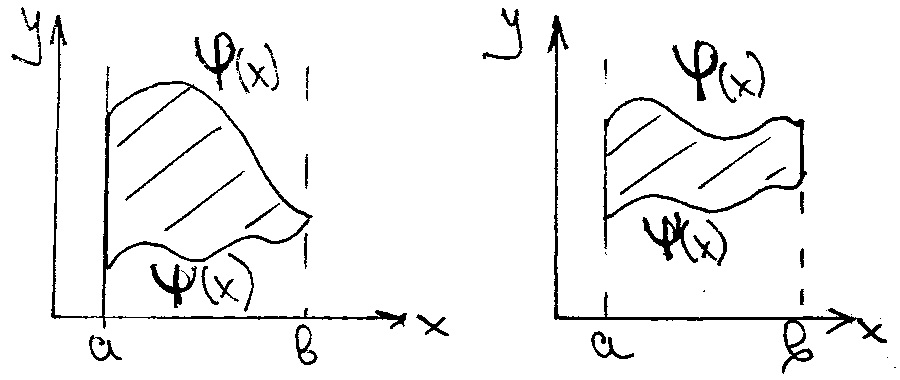
\includegraphics[width=100mm]{lect7pic1}
	\\
\end{figure}


\subsection{m-кратные интегралы}


	$\Omega \subset \mathbb{E}^m, \; Ox_1\dots x_m; \;\; \varepsilon_m \{(x_1,\dots, x_m): x_m=0\}$ где $\Omega_m $ - проекция области $\Omega$ на мн-во $\varepsilon_m$
\begin{determenition}
	Область $\Omega\subset \mathbb{E}^m$ называется \textbf{элементарной относительно $Ox_m$}, если ее проекция на $\Omega_m $ на множество $\varepsilon_m$ является областью, а  граница $\Omega$ (т.е.$ \delta\Omega$) состоит из графиков двух функций: $x_m=\phi_1(x_1,\dots, x_{m-1});\; x_m=\psi_1(x_1,\dots, x_{m-1}) $ и, быть может, боковой поверхности цилиндра, основанием которого является $\delta\Omega_m $ причем $\forall (x_1,\dots, x_{m-1})\in \overline{\Omega}_m \rightarrow  \psi(x_1,\dots, x_{m-1}) \leq \phi(x_1,\dots, x_{m-1}).$
	
\end{determenition}

\begin{theorem}
		Пусть $\omega=f(x)$ непрерывна на $\overline{\Omega} $ и область $\Omega$ элементарна относительно оси $Ox_m$, ее граница состоит из двух графиков непрерывных функций $y=\phi_1(x_1,\dots, x_{m-1});$ 
		$ y=\psi_1(x_1,\dots, x_{m-1}) $ и, быть может, боковой поверхности цилиндра оси $Ox_m $,  причем $\forall (x_1,\dots, x_{m-1})\in \overline{\Omega}_m \rightarrow  \psi_1(x_1,\dots, x_{m-1}) \leq \phi_1(x_1,\dots, x_{m-1}).$
	 	Тогда существует повторный интеграл $\underbrace{\int\dots\int}_{\Omega_m} dx_1\dots dx_{m-1} \int_{\psi_1(x_1,\dots, x_{m-1}}^{\phi_1(x_1,\dots, x_{m-1})} f(x) dx_m = \underbrace{\int\dots\int}_{\Omega_m} f(x_1, \dots, x_m)dx_1\dots dx_{m} $\\
	 	$$ \begin{cases}
	 	x=x(u,v) \\ y=y(u,v)
	 	\end{cases} 
	 	(x,y)\in\Omega; (u,v)\in\Omega^*; \; 
	 	\mathbb{J}= 
	 	\begin{vmatrix}
	 		x_u& x_v\\
	 		y_u& y_v
	 	\end{vmatrix};\;\iint\limits_\Omega f(x,y) dxdy=\iint\limits_{\Omega^*}f(x, y) | \mathbb{J}(u,v) | dudv $$
\end{theorem}

